% !TEX program=xelatex

\documentclass{scrartcl}

\usepackage{polyglossia, xltxtra}
\setmainlanguage{german}
\usepackage{amsmath,mathtools, amsthm, amssymb,cases}
\usepackage{xcolor}
\usepackage{booktabs}
\usepackage{nicefrac}
\usepackage{multirow}
\usepackage{csquotes}
\usepackage{caption}
\usepackage[loadonly]{enumitem}
\newlist{arrowlist}{itemize}{1}
\setlist[arrowlist]{label=$\Rightarrow$}

\usepackage{scrlayer -scrpage}
\lohead{Mansur Daschaew \\ Janina Rastetter \\ Maren Raus}
\cohead{Prävalenzabhängige Kontaktdaten}
\rohead{14.02.2022}
\pagestyle{scrheadings}

\graphicspath{{img/}}


%\newtheorem{defi}{Definition}[section]
%\newtheorem{satz}[defi]{Satz}
%\newtheorem{cor}[defi]{Korollar}
%\newtheorem{bem}[defi]{Bemerkung}
%\newtheorem{folg}[defi]{Folgerung}
%\newenvironment{beweis}
%	{\begin{proof}[Beweis]}
%	{\end{proof}}

\begin{document}

\begin{center}
\huge\textbf{Modellierung eines verallgemeinerten SEIR-Modells mit prävalenzabhängigen Kontaktraten}
\end{center}

\section{SEI\textcolor{gray}{D}R-Modell}

Das SEI\textcolor{gray}{D}R-Modell wird durch das folgende System gewöhnlicher Differentialgleichungen beschrieben:
\begin{align*}
\frac{dS}{dt} &= -\beta \frac{SI}{N} \\[10pt]
\frac{dE}{dt} &= \beta \frac{SI}{N} - \alpha E \\[10pt]
\frac{dI}{dt} &= \alpha E - \gamma I \textcolor{gray}{- \delta I} \\[10pt] 
\frac{dR}{dt} &= \gamma I \textcolor{gray}{+ \gamma D} \\[10pt] 
\textcolor{gray}{\frac{dD}{dt}} &\textcolor{gray}{= \delta I - \gamma D}
\end{align*}

- verallgemeintertes SEIR Modell (GG-SEIR) kann flexibleres Verhalten einbeziehen \\
- z.B. frühes sub-exponentielles Wachstum \\
- Modell beschrieben durch obige DGL, Variablen erklären \\

\section{Kontaktrate}
- Variation der Kontaktrate $\beta(t) $ \\
- $\beta(t) = \beta_0 [(1- \phi) f(t; \theta) + \phi]$ \\
- der kleinstmögliche Wert für $\beta$ ist dann $\phi\beta_0$ \\

- exponentielle, harmonische, und hyperbolische $\beta$- Funktionen, verschiedene Parameter [Plots] \\

%%%%%%%%%%%%%%%%%%%%%%%%%%%%%%%%%%%%%%%%%%%%%%%%%%%
%
% Fallbeispiel Xi'an
%
%%%%%%%%%%%%%%%%%%%%%%%%%%%%%%%%%%%%%%%%%%%%%%%%%%%

\section{Fallbeispiel Xi'an}
	\begin{itemize}
		\item Beispiel für Chinas strikte Null-Covid-Strategie
		\item Einmonatiger Lockdown ab dem 23. Dezember 2021
		\item Annahme: nicht immunisierte Bevölkerung (plausibel aufgrund relativ wirkungsloser Vakzine)
	\end{itemize}

\subsection{Strategie 1: Keine Intervention}
	Verbleibende nicht infizierte Individuen: 0.7649229\% $\Rightarrow$ Durchseuchung
	\begin{figure}[h]
        	\centering
		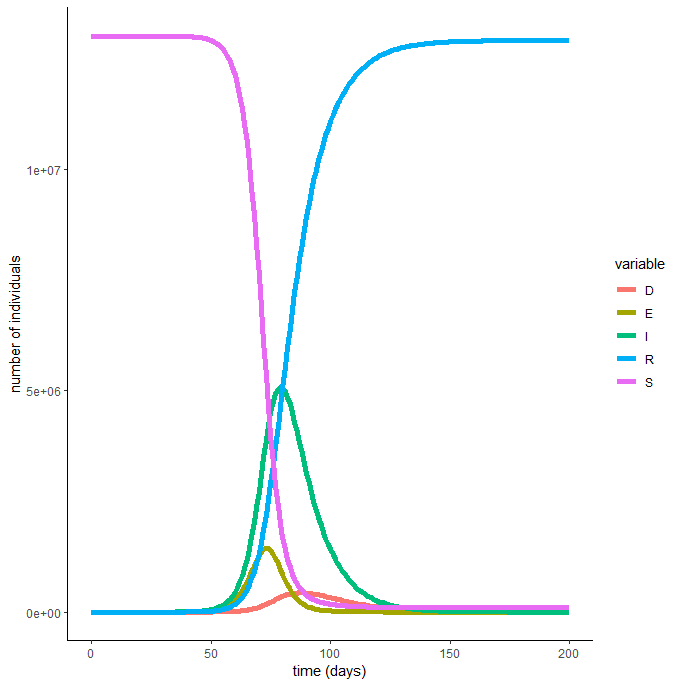
\includegraphics[scale=0.5]{delta=0,01,beta_unveraendert,alles.png}
		\caption{Verlauf mit $\delta = 0.01, \beta = \frac{5.5}{12}$}
	\end{figure}

\subsection{Strategie 2: Testen, testen, testen}
	\begin{table}[h]
		\caption{Verlauf mit verstärktem Testen}
		\centering
		\begin{tabular}{@{}ccc@{}}
			\toprule
			$\delta$ & Verbleibende S (in \%) & I und E kleiner 1, ab\\ 
			\midrule
			 $\delta_{ur} \cdot 2^1$ & 1.252596 & 212 (+ 36) \\ 
			 $\delta_{ur} \cdot 2^2$ & 2.687945 & 196 (+ 36)\\  
			 $\delta_{ur} \cdot 2^3$ & 7.447852 & 186 (+ 36)\\ 
			 $\delta_{ur} \cdot 2^4$ & 23.80182 & 211 (+ 36)\\ 
			 $\delta_{ur} \cdot 2^5$ & 76.87228 & 589 (+ 36)\\ 
			 $\delta_{ur} \cdot 2^6$ & 99.93514 & 60 (+ 36)\\ 
			\bottomrule
		\end{tabular}
	\end{table}
	\begin{figure}[h]
        	\centering
		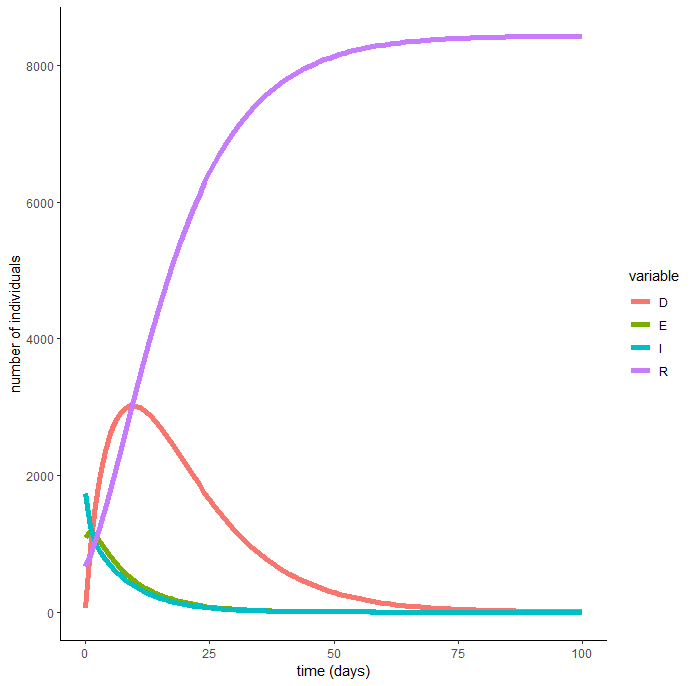
\includegraphics[scale=0.5]{delta=0,64,beta_unveraendert,ohne_s.png}
		\caption{Verlauf mit $\delta = 0.64, \beta = \frac{5.5}{12}$}
	\end{figure}	
	\begin{arrowlist}
		\item Erst ab einer Steigerung der Testeffizienz um Faktor $2^5$ ist eine Eindämmung der Epidemie möglich
		\item Bei einer Steigerung der Testeffizienz um Faktor $2^6$ müssten \enquote{nur} zwei Monate lang vermehrt getestet werden
	\end{arrowlist}

\subsection{Strategie 3: Kontaktreduktion}
	\begin{table}[h]
		\caption{Verlauf mit Kontaktreduktion}
		\centering
		\begin{tabular}{@{}ccc@{}}
			\toprule
			$\beta$ & Verbleibende S (in \%) & I und E kleiner 1, ab\\ 
			\midrule
			$\beta_{ur} * 2^{-1}$ & 11.3365 & 338 (+ 36) \\ 
			$\beta_{ur} * 2^{-2}$  & 65.28979 &  1184 (+ 36)\\  
			\nicefrac{1}{12} & 99.79345 & 898 (+ 36)\\ 
			\bottomrule
		\end{tabular}
	\end{table}
	\begin{figure}[h]
        	\centering
		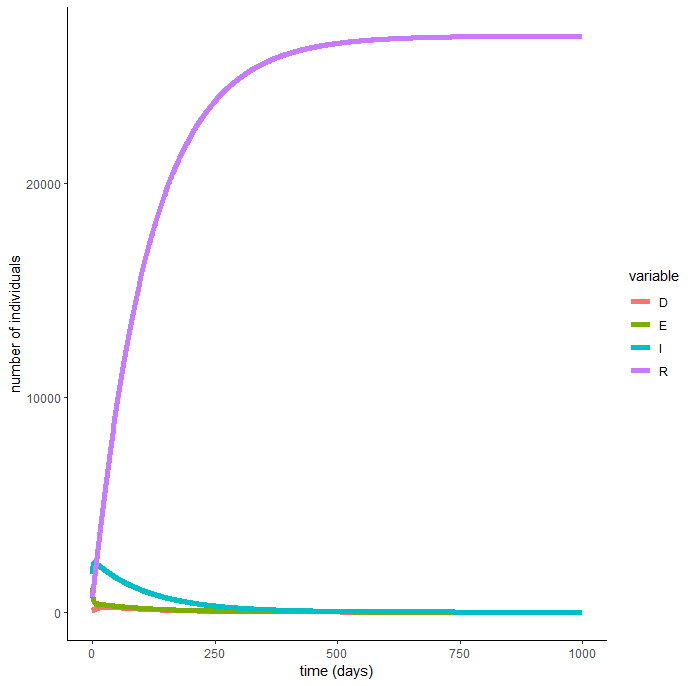
\includegraphics[scale=0.5]{delta=0,01,beta=1durch12,ohne_s.png}
		\caption{Verlauf mit $\delta = 0.0.1, \beta = \frac{1}{12}$}
	\end{figure}
	\begin{arrowlist}
		\item Kontaktreduktion verhindert Infektionen, zieht die Epidemie aber in die Länge
		\item Um eine Durchseuchung zu verhindern, müssten die Kontakte fast drei Jahre lang reduziert werden
	\end{arrowlist}

\subsection{Strategie 4: Kontaktreduktion und Massentest}
	\begin{table}[h]
		\caption{Verlauf mit verstärktem Testen und Kontaktreduktion}
		\centering
		\begin{tabular}{@{}ccc@{}}
			\toprule
			$\delta$ & Verbleibende S (in \%) & I und E kleiner 1, ab\\ 
			\midrule
			 $\delta_{ur} \cdot 2^1$ & 99.88242 & 456 (+ 36) \\ 
			 $\delta_{ur} \cdot 2^2$ & 99.92746 & 230 (+ 36)\\  
			 $\delta_{ur} \cdot 2^3$ & 99.95006 & 117 (+ 36) \\ 
			 $\delta_{ur} \cdot 2^4$ & 99.96137 & 60 (+ 36)\\ 
			 $\delta_{ur} \cdot 2^5$ & 99.96703 & 33 (+ 36)\\ 
			 $\delta_{ur} \cdot 2^6$ & 99.96986 & 20 (+ 36)\\ 
			\bottomrule
		\end{tabular}
	\end{table}
	\begin{figure}[h]
        	\centering
		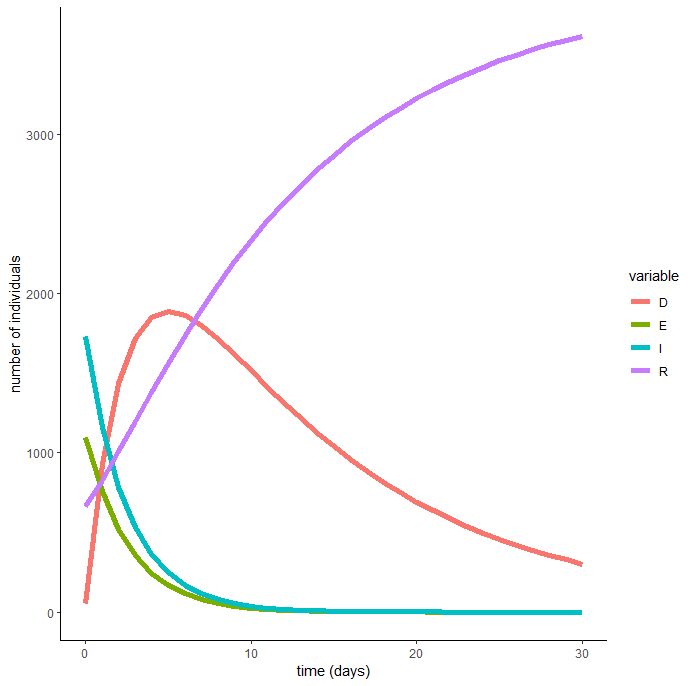
\includegraphics[scale=0.5]{delta=0,64,beta=1durch12,ohne_s.png}
		\caption{Verlauf mit $\delta = 0.64, \beta = \frac{1}{12}$}
	\end{figure}
	\begin{arrowlist}
		\item Bei extremer Kontaktreduktion wirkt sich die Testeffizienz kaum auf die Anzahl der Infektionen aus, dafür aber sehr stark auf die erforderliche Dauer der Beschränkungen
		\item Die Testeffizienz müsste mindestens um Faktor $2^4$ gesteigert werden, um die Dauer der Einschränkungen gering zu halten (ein bis zwei Monate)
	\end{arrowlist}

\subsection{Zusammenfassung}
	\begin{table}[h]
		\caption{Zusammenfassung}
		\centering
		\begin{tabular}{@{}ccccc@{}}
			\toprule
			Strategie & $\delta$ & $\beta$ & Dauer & Verbleibende S (in \%)\\ 
			\midrule
			-- & 0.01 & \nicefrac{5.5}{12} & 8.5 Monate & 0.7649229\\
			T &  0.64 & \nicefrac{5.5}{12} & 2 Monate & 99.93514\\ 
			K & 0.01 & \nicefrac{1}{12} & 2.5 Jahre & 99.79345\\
			K + T & 0.32 & \nicefrac{1}{12} & 1 Monat & 99.96703\\
			K + T & 0.64 & \nicefrac{1}{12} & 3 Wochen & 99.96986\\
			\bottomrule
		\end{tabular}
	\end{table}









\vspace*{\fill}
\textbf{Literatur:}  \\
P. Yan, G. Chowell: Quantitative Methods for Investigating Infectious Disease Outbreaks, 2019 \\
A. King: Ordinary differential equations in R, https://kinglab.eeb.lsa.umich.edu/480/nls/de.html, Zugriff: 03.02.2022

\end{document}